\documentclass[a4 122pt]{article}

\usepackage{color}
\usepackage{polski}
\usepackage[utf8]{inputenc}
\usepackage{amsmath}
\usepackage{amsthm}
\usepackage{todonotes}
\usepackage{geometry}
\usepackage{hyperref}
\geometry{
  body={6.5in, 8.5in},
  left=0.7in,
  top=0.45in,
  bottom=0.3in
}
\usepackage{graphicx} % załączanie obrazów
\usepackage{algorithm2e}
\newtheorem{twierdzenie}{Twierdzenie}
\title{Planarność grafu}
\author{Paweł Sokołowski\\Michał Kaszlej}


\begin{document}


\maketitle

	\section{Cel projektu}

		Celem projektu jest napisanie algorytmu heurystycznego sprawdzającego czy zadany graf jest planarny.
		Według twierdzenia podanego w książce (Wilson, 1998):

		\begin{figure}[h]
			\begin{center}
				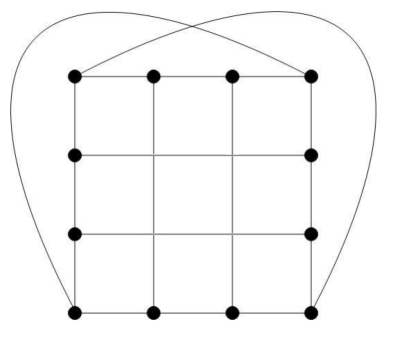
\includegraphics[width=0.5\textwidth]{include/graf.png}
				\caption{Zadany graf}
			\end{center}
		\end{figure}


		Dany graf jest planarny wtedy i tylko wtedy, gdy nie zawiera podgrafu ściągalnego do grafu $K_{3.3}$ lub do grafu $ K_5 $

	\section{Język programowania} 

		Algorytm zostanie zaimplementowany za pomocą języka C\#.

	\section{Algorytm}

		Algorytm rozwiązujący zadany problem zostanie wybrany w dalszej fazie projektu.

	\section{Opis algorytmu}	
	Algorytmem, który zostanie zaimplementowany w celu sprawdzenia czy zadany graf jest planarny jest test planarności przy użyciu twierdzeniem Wagnera. 
	Samo twierdzenie zostało już wcześniej sformułowane. 
	\begin{twierdzenie}
	Dany graf jest planarny wtedy i tylko wtedy, gdy nie zawiera podgrafu ściągalnego do grafu $K_{3.3}$ lub do grafu $ K_5 $
	\end{twierdzenie}
	Implementacja algorytmu wywodzi się wprost z powyższego twierdzenia. 
	Polegała będzie ona na dokonywaniu operacji ściągania grafu do podgrafu o 5 lub 6 wierzchołkach.
	Jeżeli uda się w ten sposób utworzyć graf $ K_5 $ lub $K_{3.3}$ oznaczało to będzie, że wejściowy graf nie jest planarny.
	Poniżej znajduje się pseudokod algorytmu.
	
	
	\begin{algorithm}[H]
	\DontPrintSemicolon
	\LinesNumbered
	\newcommand{\forcond}{$i=0$ \KwTo $n$}
	\SetKwFunction{Fn}{JestPlanarny}
	\Fn{graf g}\Begin{
	
		\KwData{Testowany graf}
		\KwResult{Czy testowany graf jest planarny}
		\If{g posiada 6 wierzchołków}{
			Sprawdź czy graf jest $K_{3.3}$\;
		}
		\If{g posiada 5 wierzchołków}{
			Sprawdź czy jest $K_5$\;
		}
		\If{graf posiada więcej niż 5 wierzchołków}{
			\ForEach{krawędź e grafu g}{
				h $\leftarrow$ zbuduj graf poprzez ściągnięcie krawędzi e z grafu g\;
				\Fn{h}\;
			}
		}
	}
	\caption{Pseudokod algorytmu}
	\end{algorithm}
	
	Linie 1-6 algorytmu wydają się dosyć oczywiste. Jeżeli mamy doczynienia z grafem pięcio lub sześcio wierzchołkowym sprawdzane 
	jest odpowiednio czy nie jest to odpowiednio $K_5$ lub $K_3.3$. W linii 8 następuje iteracja po wszystkich krawędziach grafu. 
	Najistotniejszym fragmentem algorytmu wydaje się być linia 9. Budowany jest tam nowy graf poprzez "ściągnięcie" danej krawędzi. 
	Sama operacja zostanie opisana w dalszej części pracy.
	
	\subsection{Operacja ściągnięcia}
	TODO: napisać coś
	
	\subsection{Struktury danych}
	TODO: napisać coś, wydaje mi się, że lista sąsiedztwa
	
	\subsection{Złożoność}
	
	TODO: opisać, że chyba niestety O(m!)
	
	\section{Bibliografia}

		Wilson, R. J. (1998). Wprowadzenie do teorii grafów. Warszawa: Wydawnictwo Naukowe PWN.

\end{document}	
